%% =====================================================================================
%% 6 Mixed tables, and 7 selection among agents.
%% Numbers: tables/num_mixed.tex (analysis/mixed.py), tables/num_advantage.tex
%% (analysis/advantage.py), tables/num_selection.tex (analysis/selection.py).
%% Figures: fig_advantage.pdf, fig_mixed.pdf, fig_selection.pdf.
%% Design fact, do not "fix": seat blocks are contiguous and fixed within each
%% (pair, seats) cell; the order of the two blocks alternates across cells, so every
%% model holds every seat equally often only when cells are pooled.
%% The within-table ranking follows from Proposition 2; present it as known selection
%% theory made concrete, and put the empirical weight on who pays least in company and on
%% what selection costs the group.
%% =====================================================================================
\section{Defaults in mixed groups}
\label{sec:groups}

Self-play and scripted partners cannot show what happens when agents with different defaults
share a table. We seat every pair of models together, with one to five seats for the first
model, at $p\in\{0.1,0.5,0.9\}$ and ten games per cell, for \MixGames{} games. The seats of
each model form one block whose position is fixed within a cell and alternates across cells,
so every model holds every seat equally often overall.

\begin{figure}[t]
\centering
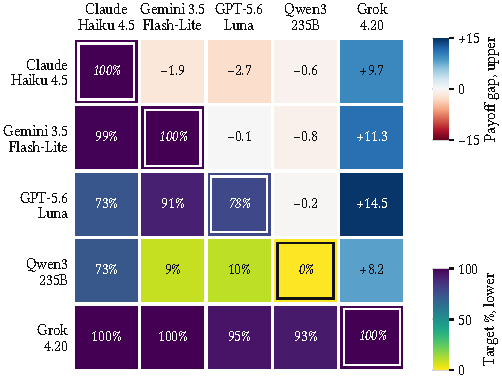
\includegraphics[width=\columnwidth]{figures/fig_advantage.pdf}
\Description{One five-by-five matrix over pairs of models, split along the diagonal. Cells
above the diagonal give the payoff of the row model's seats minus that of the column model's
seats at the same table; the Grok column is blue, meaning every other model earns more than
Grok, and the other cells are pale, meaning small differences. Cells on and below the diagonal
give the share of games that reach the target; the cells that pair Qwen with Gemini
Flash-Lite or GPT Luna are nearly white, and the Grok row is dark.}
\caption{Two models at one table, 150 games per pair, pooled over seat splits and risk. Above
the diagonal: expected payoff of the row model's seats minus the column model's, in the same
games. On and below it: share of games reaching the target; boxed cells are self-play (60
games).}
\label{fig:advantage}
\end{figure}

At a shared table every model earns more than Grok, by up to \AdvMaxAbs{} units per seat,
while the payoff gaps among the other four are small (Figure~\ref{fig:advantage}, above the
diagonal). This
follows from Proposition~\ref{prop:table}: Grok pays the most, and at one table the larger
payer earns less. Group success depends on the pair (Figure~\ref{fig:advantage}, below the
diagonal). Tables
that include Grok almost always reach the target, while tables that mix Qwen with Gemini Flash-Lite
or GPT Luna rarely do; \AdvPairLowReachName{} succeed in only \AdvPairLowReachPct\% of their
games.

\begin{figure}[t]
\centering
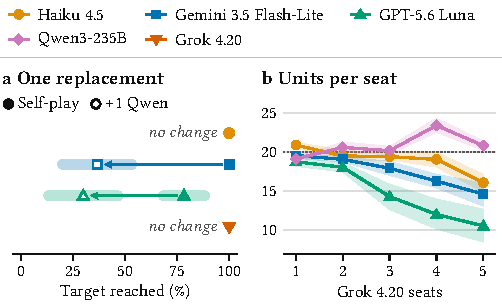
\includegraphics[width=\columnwidth]{figures/fig_mixed.pdf}
\Description{Two dot charts with one row per model, where an arrow runs from a filled marker
to an open marker. Left: the share of games reaching the target, alone and with one seat
replaced by Qwen; the arrows for Gemini Flash-Lite and GPT Luna run far to the left, while
Claude Haiku and Grok stay at full success. Right: what a seat pays beside one Grok seat and
beside five; the arrows for GPT Luna, Gemini Flash-Lite and Claude Haiku run left, below the
fair share, while Qwen moves slightly right.}
\caption{Two models at one table, pooled over $p$. Arrows run from the filled marker to the
open one, which carries a 95\% interval. (a)~Target reached by six seats of one model (60
games) and by five seats plus one Qwen seat (30). (b)~What a seat pays beside one and five Grok
seats (30 games each; dots: two to four); dotted: the fair share.}
\label{fig:mixed}
\end{figure}

\paragraph{An exact fair share has no slack.}
One partner that stops paying in the last round is enough to break a table of exact
fair-share players (Figure~\ref{fig:mixed}a). When the pool stands at 108 before round 10,
Qwen pays nothing in \MixQwenPotZeroPct\% of its decisions, against \MixFlashPotZeroPct\% for
Gemini Flash-Lite. Five Gemini Flash-Lite seats with one Qwen seat therefore succeed in only
\MixFlashQwenReach{} of 30 games, although Gemini Flash-Lite alone never misses, and five GPT
Luna seats with one Qwen seat succeed in \MixLunaQwenReach{} of 30, against
\MixLunaAloneReach\% alone. Claude Haiku and Grok tables, which pay more than needed, absorb
the same partner (\MixHaikuQwenReach{} of 30 for Claude Haiku). In \MixQwenPivotalFix\% of the
\MixMissWithQwen{} missed tables with a Qwen seat, turning its last-round zeros into 2s would
have reached the target. Slack also works the other way: one Grok seat lets five Qwen seats
reach the target in \MixGrokRescuesQwen{} of 30 games, and Grok pays for the rescue. Since
Qwen's last-round rule depends on the wording, this measures what one late dropout does to a
group, whichever model plays that role.

\paragraph{Generous partners are under-matched.}
Agents pay less, not more, when generous partners fill most of the table
(Figure~\ref{fig:mixed}b). Next to five Grok seats, GPT Luna pays \MixLunaBesideFiveGrok{} units
per seat, against \MixLunaBesideOthers{} next to other partners, and Gemini Flash-Lite and
Claude Haiku pay \MixFlashBesideFiveGrok{} and \MixHaikuBesideFiveGrok{}. As with scripted
partners, Gemini Flash-Lite and Claude Haiku stop once the pool reaches the target, while GPT
Luna pays less from the start, so the generous partner carries the group. Qwen pays slightly
more beside Grok. These responses fit watching the pool, which our design does not separate
from tracking who paid.

\section{Which agent wins under selection}
\label{sec:selection}

Systems that host many agents keep some and drop others: an operator picks the agent that
earned most, or users copy the one that did well. The key question is whom an agent is
compared with, and we show that the answer decides which of our five models such a process
favours. Following empirical game-theoretic
analysis~\cite{wellman2006methods,tuyls2018generalised}, each model is a strategy. We write
$\pi_A(k)$ for the mean expected payoff of an $A$ seat at a table with $k$ seats of $A$ and
$6-k$ seats of another model $B$, estimated from the mixed tables for $1\le k\le5$ and from
self-play for $k=6$.

\paragraph{Selection process.}
A population of $N$ agents holds $i$ agents of type $A$ and $N-i$ of type $B$, and tables of
six are drawn at random. The fitness of each type is its payoff averaged over the tables it
can land in, as given by
\begin{align}
f_A(i) &= \textstyle\sum_{k=1}^{6} \mathcal{H}(k-1;\,N-1,\,i-1)\;\pi_A(k), \label{eq:fitness}\\
f_B(i) &= \textstyle\sum_{k=0}^{5} \mathcal{H}(k;\,N-1,\,i)\;\pi_B(6-k), \nonumber
\end{align}
where $\mathcal{H}(k;\,N-1,\,m)$ is the hypergeometric chance that $k$ of the five other seats
come from the $m$ other agents of type $A$. An agent copies a random other agent with
probability $1/(1+e^{-\beta\Delta f})$, where $\Delta f$ is their fitness gap and $\beta$ is
the selection intensity, set to 1 per payoff unit. $\alpha$-Rank~\cite{omidshafiei2019alpha}
assumes that a new model enters rarely, so the population is almost always made of one model.
It computes the chance that a single newcomer takes over, for every pair of models, and turns
these chances into a Markov chain over the five one-model populations. The share of time the
chain spends on each model is the weight selection gives it, its \emph{stationary mass}. The
population size sets whom an agent is compared with. With $N=6$ the whole population is one
table, so an agent is compared only with its tablemates. With $N=30$, fitness is averaged over
random tables, so an agent is compared mostly with agents who sat elsewhere.

\paragraph{Scoring against tablemates rewards the smallest payer.}
Within one table, Proposition~\ref{prop:table} fixes the ranking before any data are seen:
the seat that pays less earns more. What the data add is who pays least in company, which is
Qwen, and what this selection costs. It gives Qwen the largest weight at every risk level
(Figure~\ref{fig:selection}, top row). The selected population then reaches the target in only
\SelWithinReachMid\% of games at $p=0.5$ and \SelWithinReachHigh\% at $p=0.9$, against
\SelUniformReachMid\% and \SelUniformReachHigh\% for a model picked at random. With stronger
selection ($\beta=\SelBetaExtra$) the success rate falls to \SelStrongWithinReachMid\% and
\SelStrongWithinReachHigh\%. This is the known result that selection on payoff relative to a
small group favours whoever does better than its neighbours, even at a cost to the
group~\cite{schaffer1988evolutionarily}, now shown with language-model agents.

\begin{figure}[t]
\centering
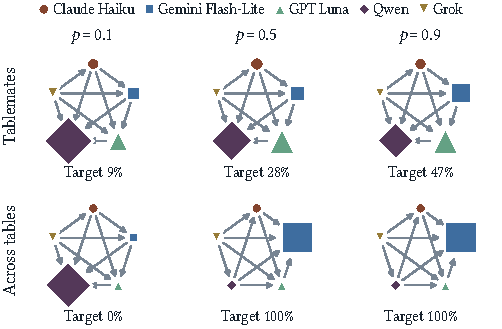
\includegraphics[width=\columnwidth]{figures/fig_selection.pdf}
\Description{Six small graphs in two rows and three columns, one column per catastrophe
probability 0.1, 0.5 and 0.9. Each graph has five nodes, one per model, arranged in a
pentagon, with arrows between every pair. Top row, comparison with tablemates: the Qwen node
is the largest at every risk level and the target rates printed below are low. Bottom row,
comparison across tables: the Qwen node is largest at 0.1, and the Gemini Flash-Lite node is
largest at 0.5 and 0.9, where the target rate is 100 percent.}
\caption{Which model selection favours ($\alpha$-Rank, $\beta=1$). A node is a one-model
population, larger when it gets more stationary mass; an arrow points to the model whose
newcomer takes over more easily. Top: $N=6$, so agents are compared with their tablemates.
Bottom: $N=30$, so mostly with agents at other tables. Under each graph: the self-play target
rate, weighted by mass.}
\label{fig:selection}
\end{figure}

\paragraph{Scoring across tables keeps the fair-share player.}
When agents are compared with agents at other tables, what matters is how well a model's own
tables do. At $p=0.5$ and $0.9$ selection then favours Gemini Flash-Lite
(Figure~\ref{fig:selection}, bottom row), whose population reaches the target in \SelAcrossReachHigh\%
of games at $p=0.9$ and earns the optimum, \SelAcrossPayHigh{} units per seat. It wins because
it is rigid: a newcomer that pays less pushes its table below the target, and one that pays
more loses money. At $p=0.1$ both rules favour \SelAcrossWinnerLow{}, which still earns far
less than the optimum, since every model pays at low risk. The winners do not change with
stronger selection, with populations of \SelNExtra{} agents, or when self-play payoffs use
only the risk grid, and each stays on top in at least \SelBootMinPct\% of bootstrap samples.
Under weak selection ($\beta=\SelWeakBeta$) no model gets more than \SelWeakWithinMaxMass{} of
the weight within a table, so the cost of tablemate scoring needs selection that is at least
moderately strong. The same
agents, scored in two reasonable ways, lead to opposite outcomes for the group, in line with
theory on selection between groups~\cite{traulsen2006evolution}, and tablemate scoring is one
simple route to the selfish outcomes that imitation produced for model-written
strategies~\cite{willis2026evaluating}.
